\documentclass{article}

\usepackage[utf8]{inputenc}
\usepackage[english]{babel}
\usepackage[margin=1in]{geometry}
\usepackage{fancyhdr}
\usepackage[hidelinks]{hyperref}
\usepackage{tikz}
\usepackage{fancyhdr}
\usepackage{float}
\usepackage{listings}
\usetikzlibrary{trees}
\author{R\'emy Detobel \& Nathan Liccardo}
\title{Report Project 1~:\\XML Schema Definition}

\usepackage{color}
\definecolor{Maroon}{rgb}{0.5,0,0}

\lstdefinelanguage{XML}
{
  basicstyle=\ttfamily\footnotesize,
  morestring=[b]",
  moredelim=[s][\bfseries\color{Maroon}]{<}{\ },
  moredelim=[s][\bfseries\color{Maroon}]{</}{>},
  moredelim=[l][\bfseries\color{Maroon}]{/>},
  moredelim=[l][\bfseries\color{Maroon}]{>},
  morecomment=[s]{<?}{?>},
  morecomment=[s]{<!--}{-->},
  commentstyle=\color{DarkOliveGreen},
  stringstyle=\color{blue},
  identifierstyle=\color{red}
}

\renewcommand\thesection{\arabic{section}}

\begin{document}

\tikzstyle{tree}=[sibling distance=10em,every node/.style = {shape=rectangle, rounded corners,draw, align=center,top color=white, bottom color=blue!20}]
\tikzstyle{optional}=[bottom color=blue!7!white]

\maketitle

\section{Introduction}
This document aims at describing and explaining all the choices that we make for this project. As a reminder, the main goal has been to create an XSD file containing a specific XML Schema Definition. This report is structured into two parts : variables and schema definitions and hypothesis. As during course lectures, we decided to use trees to represent our XSD structure.
  
  %The first part of this report will be dedicated to the structure of the schema. We will show, by means of trees, how the requested structure has been implemented. Those trees will be used to infer each specific types and links between them. The second part of this document will be focused on the hypotheses that we made during the implementation. Indeed, due to the non-formal aspect of the assignment, some parts of the structure were left to choose.
  
  
\section{Variables}
  \label{sec:variables}
This project use many different kinds of variables. Some of them are complex (see below) but most of them are simple. Simple types are : 
  \begin{itemize}
    \item \textit{String}~: title, publisher, abstract, edition, author, editor;
    \item \textit{Integer}~: volume, number, price, impact.
  \end{itemize}
Concerning the complex types, they are used for defining the year, the genre and the ISBN. As we need to declare a year using a tag or an attribute, we defined it into two parts. Firstly, we declared the format (using a simple type) and then, secondly, we defined an attribute and an element (using the year format). Genre and ISBN types are based on a restriction of the simple string type. For the first one, we have been restricted possible input (thriller, horror, sci/fi, romance, literature) using an enumeration. Finally, ISBN uses many formats (see below) that we defined using a set of patterns.
  
  \subsection{ISBN}
    \label{sec:isbn}
    % TODO
  
  
\section{Structure of the schema}
  For this project, we were assigned to write an XSD file which define a book shop. This shop is separated into two parts~: scientific products and leisure products. The following tree represent this first relation~:
  \begin{center}
    \begin{tikzpicture}[tree]
      \node {$<$bookshop$>$\\bookshop}
	child { node[optional] {$<$scientific$>$*\\ScientificProducts} }
	child { node[optional] {$<$leisure$>$*\\LeisureProducts} };
    \end{tikzpicture}
  \end{center}
  In this tree, each node contains the XML tag but also the type of the element.
  So here we can see that the ``bookshop'' type does have two children~: \verb|scientific| and \verb|leisure|. These two types will be detailed in the following points.
  Note that they are not mandatory (hence their whiter color).  The \verb|bookshop| tag may be empty or contain only one of the two types.  Note also that there can be several times the tag \verb|scientific| or \verb|leisure| (hence the star (*) next to the tag).
  
  \subsection{Scientific products}
    Scientific products are separated into two sub-categories. The first one define scientific books and the second one scientific journals. Those links can be represented as follow~:
    \begin{center}
      \begin{tikzpicture}[tree]
	\node {$<$scientific$>$\\ScientificProducts}
	  child { node[optional] {$<$book$>$*\\sciBook} }
	  child { node[optional] {$<$journal$>$*\\sciJournal} };
      \end{tikzpicture}
    \end{center}
    These two new type (sciBook and sciJournal) are a little more complex than what we have seen so far.  As \verb|bookshop|, \verb|scientific| can be empty or contain only one of the two types and here too there may be several \verb|books| or \verb|journals|.
    
    \subsubsection{Scientific book}
      \begin{center}
	\begin{tikzpicture}[tree, sibling distance=6.1em, level distance=8em]
	  \fill[blue!20!white, draw=gray, rounded corners] (-6.4,-4.1) rectangle (-2.25,-2.25);
	  
	  \node {$<$book$>$\\sciBook}
	    child { node {$<$title$>$\\titleT}}
	    child { node {$<$authors$>$\\authorsT} }
	    child { node {$<$editors$>$\\editorsT} }
	    child { node {$<$publisher$>$\\publisherT}}
	    child { node {$<$year$>$\\yearT}}
	    child { node[optional] {$<$abstract$>$\\abstractT}}
	    child { node[optional] {$<$edition$>$\\editionT}}
	    child { node[optional] {$<$ISBN$>$\\ISBNT}};
	    
	  \node[bottom color=blue!20!white, top color=blue!20!white, draw=blue!20!white] at (-4.3,-3.7) {XOR};
	\end{tikzpicture}
      \end{center}
      All types (except ``authorsT'' and ``editorsT'') have been defined previously (see point \ref{sec:variables}). The \verb|<authors>| and \verb|<editors>| tags still need to be defined. Both types contain lists of elements (respectively ``authorT'' and ``editorT''). These two types cannot appear at the same time.  Note that the last three elements are optional.
      
    \subsubsection{Scientific journal}
      \begin{center}
	\begin{tikzpicture}[tree, sibling distance=6.1em, level distance=8em]
	  \fill[blue!20!white, draw=gray, rounded corners] (-3.2,-4.1) rectangle (1,-2.25);
	  
	  \node {$<$journal$>$\\sciJournal}
	    child { node {$<$title$>$\\titleT}}
	    child { node {$<$volume$>$\\volumeT}}
	    child { node {$<$number$>$\\numberT}}
	    child { node {$<$authors$>$\\authorsT} }
	    child { node {$<$editors$>$\\editorsT} }
	    child { node {$<$year$>$\\yearT}}
	    child { node[optional] {$<$publisher$>$\\publisherT}}
	    child { node[optional] {$<$impact$>$\\impactT}}
	    child { node {$<$articles$>$\\articlesT}};
	    
	  \node[bottom color=blue!20!white, top color=blue!20!white, draw=blue!20!white] at (-1,-3.7) {XOR};
	\end{tikzpicture}
      \end{center}
      The structure is exactly the same as the previous point.  All types (except ``articlesT'') have already been defined previously.  Also as in the previous point, ``authorsT'' and ``editorsT'' cannot appear at the same time.
      
      \subsubsection{Articles}
	A scientific journal must have a list of the articles it contains.  The tag \verb|articles| therefore contains at least one tag \verb|article| which itself contains attributes.  All this can be represented by the following tree:
	\begin{center}
	  \begin{tikzpicture}[tree, sibling distance=6.1em, level distance=8em]
	    \fill[blue!20!white, draw=gray, rounded corners] (0.15,-4.7) rectangle (4.3,-2.95);
	  
	    \node {$<$articles$>$\\articlesT}[level distance=5em]
	      child {
		child { node {$<$title$>$\\titleT} }
		child { node {$<$author$>$\\authorT} }
		child { node {$<$pages$>$\\pagesT} }
		child { node {$<$number$>$\\numberT} }
		node {$<$article$>$*\\articleT}
	      };
	      
	      \node[bottom color=blue!20!white, top color=blue!20!white, draw=blue!20!white] at (2,-4.3) {XOR};
	  \end{tikzpicture}
	\end{center}
	Like \verb|authors| and \verb|editors|, \verb|pages| and \verb|number| could not appear at the same time.  The types ``titleT'', ``authorT'' and ``numberT'' have already be defined.  For ``pagesT'' it's a bit different, we must to have a start page and an end page.  Thus we have the following tree:
	\begin{center}
	  \begin{tikzpicture}[tree]
	    \node {$<$pages$>$\\pagesT}
	      child { node {$<$start$>$\\positiveInteger} }
	      child { node {$<$end$>$\\positiveInteger} };
	  \end{tikzpicture}
	\end{center}
	
      \subsubsection{Impact}
	As indicated in section \ref{sec:variables}, the ``impact'' type is an integer calculated according to the number of citations, received in that year, of articles published in that journal during the two preceding years, divided by the total number of articles published in that journal during the two preceding years.\\
	We can therefore see that the impact is different each year and that these two data are inseparable. The impact is characterized by an ``year'' attribute (which is ``yearType'').\\
	Concretely in XML we can read this:
	\begin{lstlisting}[language=XML]
<impact year="XXXX"> ... </impact>
	\end{lstlisting}

  \subsection{Leisure products}
    The second section of a book shop is dedicated to leisure products. As for scientific one, products are separated into two sub-categories. The first one is used to define leisure books and the second one leisure periodicals. Once again, those links can be illustrated by means of a tree~:
    \begin{center}
      \begin{tikzpicture}[tree]
	\node {$<$leisure$>$\\LeisureProducts}
	  child { node[optional] {$<$book$>$*\\leiBook} }
	  child { node[optional] {$<$periodical$>$*\\leiPeriodical} };
      \end{tikzpicture}
    \end{center}
    
    \subsubsection{Leisure Book}
      \begin{center}
	\begin{tikzpicture}[tree, sibling distance=6.5em, level distance=8em]
	  \node {$<$book$>$\\leiBook}
	    child { node {$<$title$>$\\titleT} }
	    child { node {$<$authors$>$\\authorsT} }
	    child { node {$<$publisher$>$\\publisherT} }
	    child { node {$<$year$>$\\yearT} }
	    child { node {$<$genre$>$\\genreT} }
	    child { node[optional] {$<$edition$>$\\editionT} }
	    child { node[optional] {$<$number$>$\\numberT} };
	\end{tikzpicture}
      \end{center}
      All the types presented in the tree above have already been defined.
    
    \subsubsection{Periodical Leisure}
      \begin{center}
	\begin{tikzpicture}[tree]
	  \node {$<$periodical$>$\\leiPeriodical}
	    child { node {$<$title$>$\\titleT} }
	    child { node {$<$price$>$\\priceT} }
	    child { node {$<$publisher$>$\\publisherT} };
	\end{tikzpicture}
      \end{center}
      Here too, everything has already been defined previously.
    
\section{Old part}
\begin{center}
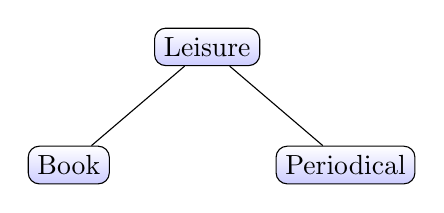
\begin{tikzpicture}[sibling distance=10em,
  every node/.style = {shape=rectangle, rounded corners,
    draw, align=center,
    top color=white, bottom color=blue!20}]]
  \node {Leisure}
    child { node {Book} }
    child { node {Periodical} };
\end{tikzpicture}
\end{center}
Following this tree, we can obtain two relations. These last are used to define an abstract bookshop (bookshopType) and a final leisure (leisureType). Finally, we obtain the next definitions :
\begin{itemize}
\item bookshopType $\rightarrow$ (leisure, leisureType)
\item leisureType $\rightarrow$ (book, booktype2), (periodical, periodicalType)
\end{itemize}
As said in the previous sub-section, bookshopType is actually not completely defined. For this reason, there exist some incompatibilities between the scientific and leisure part. Notice that leisure books and scientific books are not using same types. In fact we will see in the next section that they have two different definitions.

\subsection{Complete schema}
The two previous parts were focused on the scientific and leisure definitions. We have now to merge those definitions to obtain the final tree. In fact, a bookshop is a combination of scientific and leisure products. Notice that for each element (book, journal, ...) we can also have multiple instances of it. Finally, we obtain the following tree :
\begin{center}
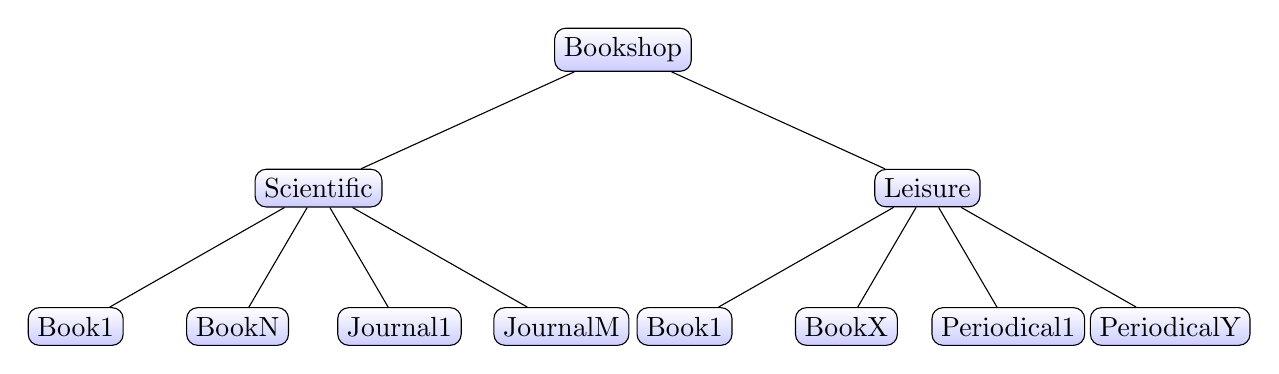
\begin{tikzpicture}[level distance=5em,
	level 1/.style={sibling distance=22em},
  level 2/.style={sibling distance=5.85em},
  every node/.style = {shape=rectangle, rounded corners,
    draw, align=center,
    top color=white, bottom color=blue!20}]]
  \node{Bookshop}  
    child { node {Scientific}
    	child { node {Book1} }
	child { node {BookN} }
    	child { node {Journal1} }
	child { node {JournalM} } }  
    child { node {Leisure}
    	child { node {Book1} }
    	child { node {BookX} }
    	child { node {Periodical1} }
    	child { node {PeriodicalY} } };
\end{tikzpicture}
\end{center}
Previously, we defined the bookshopType as an abstract one. In fact, this type was a sequence of scientificType and leisureType and could not be defined in one time. As we changed the definition of a bookshopType but also of a scientificType and a leisureType, we obtain three new relations :
\begin{itemize}
\item bookshopType $\rightarrow$ (scientific, scientificType),(leisure, leisureType)
\item scientificType $\rightarrow$ (book, booktype1)*, (journal, journalType)*
\item leisureType $\rightarrow$ (book, booktype2)*, (periodical, periodicalType)*
\end{itemize}
For the moment, we only defined links between elements. All those are created by defining complex types with some elements inside. Each of these elements are themselves referring to other complex type excepted for final types (Book, Journal, ...). The second part of this report will be focused on explaining and illustrating all the choices that we made during the implementation. For this reason, we will also detail the structure of each final types.

\section{Hypotheses and choices}
All along the previous section, we only described the global structure of the schema. We will now focus on what we called previously "final types". There exist four different kinds of this specific element : bookType1, journalType, bookType2 and periodicalType. As said in the previous section, bookType1 and bookType2 are both identified by the \verb|<book>| tag but are not referring to the same type. This can be achieved due to the scope definition. In fact, bookType1 is defined inside the scientific scope unlike bookType2 which is defined inside the leisure scope. Regarding to the two last types, journalType is identified by the \verb|<journal>| tag (scientific scope) and periodicalType by the \verb|<periodical>| tag (leisure scope). This section will be separated into two sub-sections : the XSD's structure and the final types structures.

\subsection{XSD's structure}
Our file has been split into five distinct parts. Each part is used to represent one level of the XML Schema. Indeed, the order of declarations is made from bottom to top level. Here is the used structure :
\begin{enumerate}
\item Simple types : This first section is used to define each atomic elements. This is mainly useful to reduce duplicate definitions and code. For example, we define the title element, the publisher element, etc.
\item Scientific part : Define all complex types which belong to the scientific product tree. We can see that scientificBook and scientificJournal are defined at the end of this section. Detail about this part will be given in the next section.
\item Leisure part : As the scientific part, leisure part is used to define all complex types which belong to the leisure tree. Once again, details about this part will be given later.
\item Products part : Define two complex types, scientific product and leisure product. Both can be seen as root elements from the two previous parts.
\item Bookshop part : Is used to merge both products elements. This section also define the root element of the xml file named \verb|<b:bookshop>|.
\end{enumerate}

\subsection{Final types}
This second section will be focused on the structure of each final types. As said before, there exist four different final types : bookType1, journalType, bookType2 and periodicalType.

\subsubsection{BookType1}
According to the assignment, a scientific book must be composed of : a title, a list of authors xor a list of editors, a publisher and a year of publication. Optionally, a book can have : an abstract, an edition and an ISBN. Formally, we obtain the following definition :
\begin{itemize}
\item bookType1 $\rightarrow$ (title, titleT), (authors, authorsT)$^+$ $|$ (editors, editorsT)$^+$, (publisher, publisherT), (year, yearT), (abstract, abstractT)?, (edition, editionT)?, (ISBN, ISBNT)?
\end{itemize}
All the types, excepted authorsT and editorsT, used in the previous section are defined in the simple types section. Regarding to authorsT and editorsT, their definitions are more complex. Indeed, they are themselves complex types definitions. We made the arbitrary choice that a list of authors (or editors) must be structured as follow : 
\begin{lstlisting}[language=XML]
    <authors>
	<author> ... </author>
	....
	<author> ... </author>
    </author>
\end{lstlisting}
Which implies that author and editor tags are defined by authorT and editorT. These new types are finally defined in the simple type section (as string elements).
\subsubsection{JournalType}
A scientific journal as also two parts : a mandatory one and an optional one. For the mandatory part, we must have : a title, a volume, a number, a list of authors xor a list of editors and a year. Concerning to the optional part, a journal type can have a publisher and an impact. In addition, a journal must also have a list of articles. Finally, we obtain this relation :
\begin{itemize}
\item journalType $\rightarrow$ (title, titleT), (volume, volumeT), (number, numberT), (authors, authorsT)$^+$ $|$ (editors, editorsT)$^+$, (year, yearT), (publisher, publisherT)?, (impact, impactT)?, (articles, articlesT)
\end{itemize}
Were we have two new complex types : impact and article. All the other one are defined in the simple type section excepted editors and authors which were defined previously. An impact is defined with two elements namely a year and an impact factor. For this reason, we decided to structure this complex type as follow :
\begin{lstlisting}[language=XML]
    <impact year="XXXX"> ... </impact>
\end{lstlisting}
Notice that another solution was to create a complex type (impact) composed by a year tag and a factor tag. Regarding to the articles type, we had to define a list of articles. To do that, we defined a complex type composed itself by a list of article tags. Here is the XML logic : 
\begin{lstlisting}[language=XML]
    <articles>  
    	<article> ... </article>
	...
	<article> ... </article>
    </articles>
\end{lstlisting}
Inside each article, we must find those elements : a title, an author, an interval of pages xor a number corresponding to the article. This can be formalised by the following relation : 
\begin{itemize}
\item articlesT $\rightarrow$ (article, articleT)$^+$
\item articleT $\rightarrow$ (title, titleT), (author, authorT), (pages, pagesT) $|$ (number, numberT)
\end{itemize}
Note that this type contains only one author but also that we use the complex type pagesT and the simple type numberT (define in the first section). PagesT is a very simple complex type composed of two integers corresponding to the start and end page.
\subsubsection{BookType2}
The second book type is defined inside the leisure scope. For this reason, the composition of this new book type will differ from bookType1. Inside this new book type we must find : a title, a list of authors, a publisher, a year and a genre. Optionally, we can add  an edition and a number. Formally, we obtain the following relation :
\begin{itemize}
\item bookType2 $\rightarrow$ (title, titleT), (authors, authorsT), (publisher, publisherT), (genre, genreT), (edition, editionT)?, (number, numberT)?
\end{itemize}
We were asked to restrict the value of a genre. To do that we used a restriction tag with multiple enumerations inside. All the other types were defined previously or are defined in the simple type section.
\subsubsection{PeriodicalType}
This last complex type is only composed by a sequence of three simple type elements. As these elements are very simple, we will not give any more informations about them. Here is the formal definition of a periodicalType :
\begin{itemize}
\item periodicalType $\rightarrow$ (title, titleT), (price, priceT), (publisher, publisherT)
\end{itemize}

\subsection{Complete schema and relations}
To complete this report, we can now show all the relations corresponding to the final tree. Note that those relations are now correctly named (as same as in the XSD file) and that we order relations from top to bottom (reverse file order). Due to their trivial aspects, we didn't add simple type (texts, numbers, ...)
\begin{center}
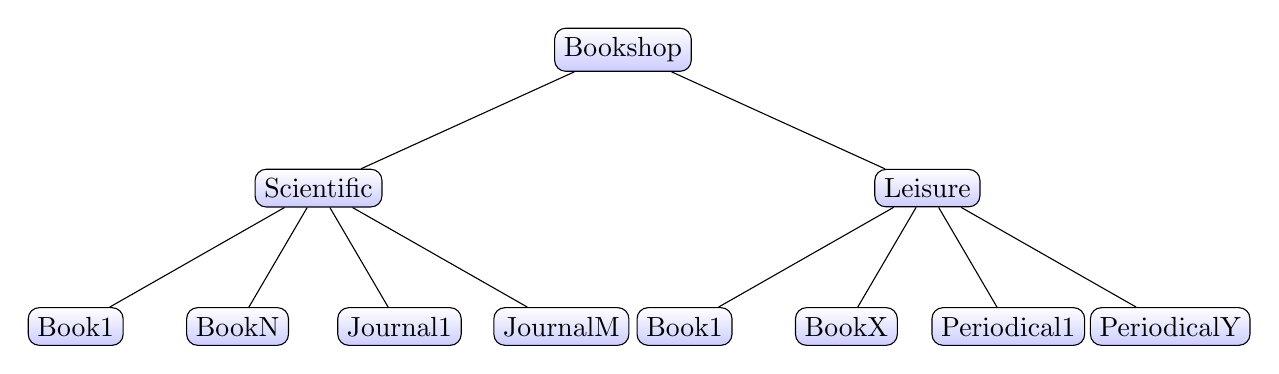
\begin{tikzpicture}[level distance=5em,
	level 1/.style={sibling distance=22em},
  level 2/.style={sibling distance=5.85em},
  every node/.style = {shape=rectangle, rounded corners,
    draw, align=center,
    top color=white, bottom color=blue!20}]]
  \node{Bookshop}  
    child { node {Scientific}
    	child { node {Book1} }
	child { node {BookN} }
    	child { node {Journal1} }
	child { node {JournalM} } }  
    child { node {Leisure}
    	child { node {Book1} }
    	child { node {BookX} }
    	child { node {Periodical1} }
    	child { node {PeriodicalY} } };
\end{tikzpicture}
\end{center}
\begin{itemize}
\item bookshopType $\rightarrow$ (scientific, scientificType),(leisure, leisureType)
\item scientificType $\rightarrow$ (book, booktype1)*, (journal, journalType)*
\item leisureType $\rightarrow$ (book, booktype2)*, (periodical, periodicalType)*
\item bookType1 $\rightarrow$ (title, titleT), (authors, authorsT)$^+$ $|$ (editors, editorsT)$^+$, (publisher, publisherT), (year, yearT), (abstract, abstractT)?, (edition, editionT)?, (ISBN, ISBNT)?
\item journalType $\rightarrow$ (title, titleT), (volume, volumeT), (number, numberT), (authors, authorsT)$^+$ $|$ (editors, editorsT)$^+$, (year, yearT), (publisher, publisherT)?, (impact, impactT)?, (articles, articlesT)
\item articlesT $\rightarrow$ (article, articleT)$^+$
\item articleT $\rightarrow$ (title, titleT), (author, authorT), (pages, pagesT) $|$ (number, numberT)
\item bookType2 $\rightarrow$ (title, titleT), (authors, authorsT), (publisher, publisherT), (genre, genreT), (edition, editionT)?, (number, numberT)?
\item periodicalType $\rightarrow$ (title, titleT), (price, priceT), (publisher, publisherT)
\end{itemize}


\newpage
\appendix

\section{Global Schema}
  \begin{center}
    \begin{tikzpicture}[tree]
      %\fill[blue!20!white, draw=gray, rounded corners] (0.15,-4.7) rectangle (4.3,-2.95);
    
      \node {$<$bookshop$>$\\bookshop}
	child { 
	  child { 
	    node[optional] {$<$book$>$*\\sciBook} 
	  }
	  child { 
	    node[optional] {$<$journal$>$*\\sciJournal} 
	  }
	  node[optional] {$<$scientific$>$*\\ScientificProducts} 
	}
	child { 
	  child { 
	    node[optional] {$<$book$>$*\\leiBook} 
	  }
	  child { 
	    node[optional] {$<$periodical$>$*\\leiPeriodical} 
	  }
	  node[optional] {$<$leisure$>$*\\LeisureProducts} 
	};
    
      %\node {$<$articles$>$\\articlesT}[level distance=5em]
	%child {
	 % child { node {$<$title$>$\\titleT} }
	  %child { node {$<$author$>$\\authorT} }
	  %child { node {$<$pages$>$\\pagesT} }
	  %child { node {$<$number$>$\\numberT} }
	  %node {$<$article$>$*\\articleT}
	%};
	
	%\node[bottom color=blue!20!white, top color=blue!20!white, draw=blue!20!white] at (2,-4.3) {XOR};
    \end{tikzpicture}
  \end{center}

\end{document}